\documentclass[12pt]{article}
\usepackage{graphicx} % Required for inserting images
\usepackage{hyperref}
\usepackage{makecell}
\usepackage{makeidx}
\usepackage{eurosym}
\usepackage{fancyhdr}
\usepackage{titlesec}
\newcommand{\firstPage}{
    \thispagestyle{empty}
    \begin{figure}
    \centering
    
\includegraphics[scale=0.7]{Swellfish_logo.png}
    \end{figure}
    \author{
        \date{}
        \href{mailto://swellfish14@gmail.com}{swellfish14@gmail.com} \\
    } 
} 
\usepackage{hyperref}
\usepackage{array}
\usepackage{tabularx}
\usepackage{adjustbox}

\newcounter{verscount}
\setcounter{verscount}{0}
\newcommand{\addversione}[5]{
	\ifdefined\setversione
		\setversione{#1}
	\else\fi
	\stepcounter{verscount}
	\expandafter\newcommand%
		\csname ver\theverscount \endcsname{#1&#2&#3&#4&#5}
}

\newcommand{\listversioni}{
	\ifnum\value{verscount}>1
		\csname ver\theverscount \endcsname
		\addtocounter{verscount}{-1}
		\\\hline
		\listversioni
	\else
		\csname ver\theverscount \endcsname\\\hline
	\fi
}

\newcommand{\makeversioni}{
	\begin{center}
		\begin{tabularx}{\textwidth}{|c|c|X|X|X|}
		\hline
		\textbf{Versione} & \textbf{Data} & \textbf{Redattore} & \textbf{Verificatore} & \textbf{Descrizione} \\
		\hline
		\listversioni
		\end{tabularx}
	\end{center}
	\clearpage
}

\fancypagestyle{genericDocstyle}{
	\pagestyle{fancy}
	\lhead{
\includegraphics[width=1cm]{Swellfish_logo.png}}
	\rhead{Norme di progetto}
}

%\hypersetup{colorlinks=true,urlcolor=blue}

%\newcommand{\tableContent}{

	%{
		%\hypersetup{linkcolor=black}
		%\tableofcontents
	%}
%}
\begin{document}
\graphicspath{ {../templates/img/} }
\setcounter{tocdepth}{4}
\setcounter{secnumdepth}{4}
\title{Piano di progetto}

\firstPage

\pagestyle{genericDocstyle}
\maketitle

\begin{center}
    \begin{tabular}{r | l}
		\multicolumn{2}{c}{\textit{Informazioni}}\\
		\hline
		
			\textit{Redattori} &
			[Davide Porporati, Elena Marchioro, Francesco Naletto]\makecell{}\\

			\textit{Revisori} &
			[Jude Vensil Barceros]\makecell{}\\
			\textit{Responsabili} &
			[Andrea Veronese]\makecell{}\\
		      \textit{Uso} & 
                [Esterno]\makecell{}\\
    \end{tabular}
\end{center}

\begin{center}
    \textbf{Descrizione}\\
    File contenente il piano di progetto per la valutazione dei costi e del raggiungimento delgi obiettivi.
\end{center}

\pagebreak

\tableofcontents
\pagebreak

\printindex 
\pagebreak

\tableofcontents
\pagebreak

\printindex 

\addversione{0.0.0}{25/04/2023}{Davide Porporati, Elena Marchioro, Francesco Naletto}{Jude Vensil Barceros}{Creata struttura di base del documento}
\addversione{0.0.1}{27/04/2023}{Davide Porporati, Elena Marchioro, Francesco Naletto}{Jude Vensil Barceros}{Aggiunto diagramma e tabella suddivisione ore}
\addversione{0.0.2}{28/04/2023}{Davide Porporati, Elena Marchioro, Francesco Naletto}{Jude Vensil Barceros}{Aggiunto resoconto primo sprint}
\addversione{0.0.3}{04/05/2023}{Elena Marchioro, Francesco Naletto, Jude Vensil Barceros}{Andrea Veronese}{Aggiunto resoconto secondo sprint e problematiche riscontrate}
\addversione{0.0.4}{11/05/2023}{Francesco Naletto, Jude Vensil Barceros, Andrea Veronese}{Claudio Giaretta}{Aggiunto resoconto terzo sprint}
\makeversioni

\section{Introduzione}
Lo scopo di questo documento è quello di fornire un riepilogo del lavoro svolto, del tempo impiegato e dei costi sostenuti, stilato ad intervalli regolari.
Questo documento conterrà una sintesi degli sprint effettuati, con le relative tabelle del costo orario e monetario sostenuto.

\section{Pianificazione Generale}
\subsection{Diagramma di Gantt}
Viene qui inserito il diagramma di Gantt, contenente la percentuale di completamento delle varie attività svolte al momento delle redazione.
\begin{center}
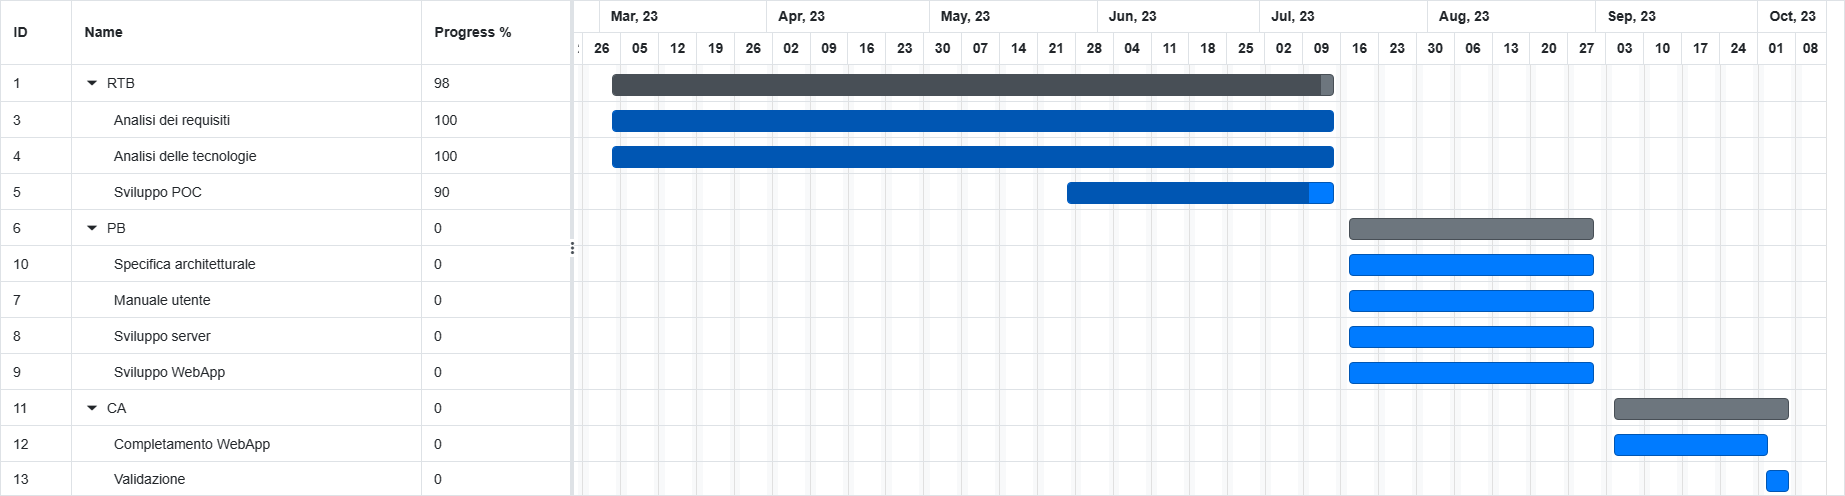
\includegraphics[width=1.2\textwidth]{Gantt}
\end{center}

\subsection{Preventivo ore finale}
In questa sezione viene riportato il preventivo orario stimato all'inizio delle attività del progetto. Al termine delle attività verrà valutato se tale preventivo è stato rispettato o meno, fornendo un'analisi dettagliata delle motivazioni che hanno portato all'eventuale superamento delle stime.
\begin{center}  
    \begin{tabular}{|l|l|l|l|}
        \hline
        \textbf{Ruolo} & \textbf{Costo orario} & \textbf{Ore Preventivate} & \textbf{Costo totale}\\
        \hline
        Responsabile & 30 & 63 & 1890\euro  \\ 
        \hline
        Amministratore & 20 & 65 & 1300\euro \\
        \hline
        Analista & 25 & 88 & 2200\euro \\
        \hline
        Progettista & 25 & 120 & 3000\euro \\
        \hline
        Programmatore & 15 & 135 & 2025\euro \\
        \hline
        Verificatore & 15 & 99 & 1485\euro \\
        \hline
        \textbf{Totale} &  & \textbf{570} & \textbf{11900\euro} \\
        \hline
    \end{tabular}
\end{center}

Viene riportata anche la suddivisione delle ore tra i membri preventivata all'inizio delle attività:
\begin{center}  
    \begin{tabular}{|l|l|l|l|l|l|l|}
        \hline
        \textbf{Nome} & \textbf{RS} & \textbf{AM} & \textbf{AL} & \textbf{PG} & \textbf{PT} & \textbf{VR}\\
        \hline
        Andrea Veronese & 11 & 11 & 16 & 17 & 23 & 17  \\
        \hline
        Claudio Giaretta & 11 & 11 & 13 & 22 & 23 & 15\\
        \hline
        Elena Marchioro & 12 & 10 & 14 & 21 & 22 & 16 \\
        \hline
        Davide Porporati & 10 & 9 & 16 & 19 & 22 & 19 \\
        \hline
        Francesco Naletto & 9 & 13 & 14 & 21 & 22 & 16 \\
        \hline
        Jude Vensil Barceros & 10 & 11 & 15 & 20 & 23 & 16 \\
        \hline
        \textbf{Totale/Ruolo} & 63 & 65 & 88 & 120 & 135 & 99 \\
        \hline
    \end{tabular}
\end{center}
\subsection{Preventivo a finire}
Al termine delle attività verrà effettuata un'analisi mirata a capire le motivazioni che abbiano portato ad uno sforamento delle ore e/o dei costi.
\subsection{Stato d'avanzamento corrente}
Attualmente il gruppo sta effettuando attività di analisi dei requisiti e di consolidamento del way of working. La documentazione viene aggiornata di pari passo con i progressi effettuati, come testimoniato dalle sottoversioni e dalla tabella delle modifiche effettuate.
\section{Metodo di Lavoro}
Il gruppo ha concordato l'utilizzo del framework Scrum come metodo di lavoro agile. 
Riportiamo per intero le caratteristiche di ogni "$sprint$": 
\begin{itemize}
    \item Durata sprint: una settimana. L'inizo dello sprint è stato concordato al venerdì, mentre il venerdì successivo verrà effettuata una riunone per capire quali obbiettivi siano stati completati e in che metodo.
    \item Ruoli: i ruoli dei membri vengono fatti ruotare settimanalmente, così da garantire un continuo cambiamento di responsabilità.
    \item Obiettivi da completare: vengono decisi prima dell'inizio dello sprint e vengono riportati nella board "$SwellFish$".
\end{itemize}
E' stato previsto che alcuni sprint non vadano a buon fine a causa di difficoltà varie, pertanto non avendo centrato tutti gli obiettivi si valuterà lo stato di avanzamento di quelli iniziati ma non completati.

\section{Sprint Scrum}
\section{Sprint 0}
Qui vengono riportate le informazioni relative al primo sprint del gruppo. Questo primo ciclo è caratterizzato dallo svolgimento di attività prettamente documentali e di analisi dei requisiti, pertanto come concordato tra i membri del team i ruoli di analista e programmatore non sono stati impiegati.

Caratteristiche:
\begin{itemize}
    \item Data inizio: 21/04/2023
    \item Data fine preventivata: 28/04/2023
    \item Data fine effettiva: 28/04/2023
\end{itemize}
\subsection{Pianificazione}
\begin{center}
    \begin{tabularx}{\textwidth}{|X|X|}
        \hline
        \multicolumn{2}{|c|}{\textbf{Item da realizzare}}\\
        \hline
        \hline
        \textbf{Item} & \textbf{Persone richieste}\\
        \hline
        Piano di progetto & 1\\
        \hline
        Piano di qualifica & 1\\
        \hline
        Norme di progetto & 2\\
        \hline
        Analisi dei requisiti & 2 \\
        \hline
    \end{tabularx}\\[8pt]
    \mbox{}\\
\end{center}
\subsection{Preventivo Costi/Ore}
\begin{center}
    \begin{tabularx}{\textwidth}{|X|X|X|X|}
        \hline
        \multicolumn{4}{|c|}{\textbf{Preventivo ore/costi}}\\
        \hline
        \hline
        \textbf{Ruolo} & \textbf{Costo orario (\euro)} & \textbf{Ore} & \textbf{Prezzo (\euro)}\\
        \hline
        Responsabile    & 30 & 5  & 150\\
        \hline
        Amministratore  & 20 & 5  & 100\\
        \hline
        Analista        & 25 & 15  & 375\\
        \hline
        Progettista     & 25 & 0  & 0\\
        \hline
        Programmatore   & 15 & 0  & 0\\
        \hline
        Verificatore    & 15 & 4  & 60\\
        \hline
        \hline
        \textbf{Totale} &    & 29 & 685\\
        \hline
    \end{tabularx}\\[8pt]
    \mbox{}\\
\end{center}
\subsection{Problematiche riscontrate}
Al termine del primo sprint non sono state rilevate particolari problematiche, pertanto questa sezione non ne riporta.
\subsection{Resoconto}
\begin{center}
    \begin{tabularx}{\textwidth}{|X|X|X|X|}
        \hline
        \multicolumn{4}{|c|}{\textbf{Preventivo ore/costi}}\\
        \hline
        \hline
        \textbf{Ruolo} & \textbf{Costo orario (\euro)} & \textbf{Ore} & \textbf{Prezzo (\euro)}\\
        \hline
        Responsabile    & 30 & 7(+7)  & 210\\
        \hline
        Amministratore  & 20 & 5(+5)  & 100\\
        \hline
        Analista        & 25 & 12(+12)  & 300\\  
        \hline
        Progettista     & 25 & 0(+0)  & 0\\
        \hline
        Programmatore   & 15 & 0(+0)  & 0\\
        \hline
        Verificatore    & 15 & 4(+4)  & 60\\
        \hline
        \hline
        \textbf{Totale} &    & 28 & 670\\
        \hline
    \end{tabularx}\\[8pt]
    \mbox{}\\
\end{center}


\section{Sprint 1}
Qui vengono riportate le informazioni relative al secondo sprint del gruppo. \\
Il secondo ciclo è stato caratterizzato dalla revisione completa delle norme di progetto e dalla revisione degli user case fino ad ora incontrati nell'analisi dei requisiti.\\
Oltre a ciò, è stato realizzato il template da utilizzare per i diari di bordo.


Caratteristiche:
\begin{itemize}
    \item Data inizio: 27/04/2023
    \item Data fine preventivata: 05/05/2023
    \item Data fine effettiva: 04/05/2023
\end{itemize}
\subsection{Pianificazione}
\begin{center}
    \begin{tabularx}{\textwidth}{|X|X|}
        \hline
        \multicolumn{2}{|c|}{\textbf{Item da realizzare}}\\
        \hline
        \hline
        \textbf{Item} & \textbf{Persone richieste}\\
        \hline
        Piano di progetto & 1\\
        \hline
        Norme di progetto & 3\\
        \hline
        Analisi dei requisiti & 2 \\
        \hline
    \end{tabularx}\\[8pt]
    \mbox{}\\
\end{center}
\subsection{Preventivo Costi/Ore}
\begin{center}
    \begin{tabularx}{\textwidth}{|X|X|X|X|}
        \hline
        \multicolumn{4}{|c|}{\textbf{Preventivo ore/costi}}\\
        \hline
        \hline
        \textbf{Ruolo} & \textbf{Costo orario (\euro)} & \textbf{Ore} & \textbf{Prezzo (\euro)}\\
        \hline
        Responsabile    & 30 & 5  & 150\\   
        \hline
        Amministratore  & 20 & 4  & 80\\ 
        \hline
        Analista        & 25 & 9  & 225\\ 
        \hline
        Progettista     & 25 & 0  & 0\\
        \hline
        Programmatore   & 15 & 0  & 0\\
        \hline
        Verificatore    & 15 & 4  & 60\\
        \hline
        \hline
        \textbf{Totale} &    & 22 & 515\\
        \hline
    \end{tabularx}\\[8pt]
    \mbox{}\\
\end{center}
\subsection{Problematiche riscontrate}
L'unica problematica riscontrata fino ad ora è stata quella della ristrutturazione delle norme di progetto, pertanto è stato dedicato del tempo aggiuntivo per ristrutturare e incrementare il way of working seguendo il ciclo di vita del software.
L'aggiunta degli UML per gli Use Case è stata rimandata al prossimo sprint per approfondire al meglio il loro funzionamento e perchè lo sprint è durato un giorno in meno a causa della coincidenza con il diario di bordo.
\subsection{Resoconto}
\begin{center}
    \begin{tabularx}{\textwidth}{|X|X|X|X|}
        \hline
        \multicolumn{4}{|c|}{\textbf{Preventivo ore/costi}}\\
        \hline
        \hline
        \textbf{Ruolo} & \textbf{Costo orario (\euro)} & \textbf{Ore} & \textbf{Prezzo (\euro)}\\
        \hline
        Responsabile    & 30 & 12(+5)  & 150\\
        \hline
        Amministratore  & 20 & 9(+4)  & 80\\
        \hline
        Analista        & 25 & 21(+9)  & 225\\
        \hline
        Progettista     & 25 & 0(+0)  & 0\\
        \hline
        Programmatore   & 15 & 0(+0)  & 0\\
        \hline
        Verificatore    & 15 & 8(+4)  & 60\\
        \hline
        \hline
        \textbf{Totale} &    & 50 &  1185 \\
        \hline
    \end{tabularx}\\[8pt]
    \mbox{}\\
\end{center}


\section{Sprint 2}
Qui vengono riportate le informazioni relative alla terza settimana di sprint del gruppo. \\
Il terzo ciclo è stato caratterizzato dal perfezionamento dell'analisi dei requisiti, individuando nuovi casi d'uso non considerati in precedenza ed espandendoli con la rappresentazione tramite UML.\\



Caratteristiche:
\begin{itemize}
    \item Data inizio: 04/04/2023
    \item Data fine preventivata: 11/05/2023
    \item Data fine effettiva: 11/05/2023
\end{itemize}

\subsection{Pianificazione}
\begin{center}
    \begin{tabularx}{\textwidth}{|X|X|}
        \hline
        \multicolumn{2}{|c|}{\textbf{Item da realizzare}}\\
        \hline
        \hline
        \textbf{Item} & \textbf{Persone richieste}\\
        \hline
        Piano di progetto & 1\\
        \hline
        Piano di qualifica & 2\\
        \hline
        Analisi dei requisiti & 3 \\
        \hline
    \end{tabularx}\\[8pt]
    \mbox{}\\
\end{center}
\subsection{Preventivo Costi/Ore}
\begin{center}
    \begin{tabularx}{\textwidth}{|X|X|X|X|}
        \hline
        \multicolumn{4}{|c|}{\textbf{Preventivo ore/costi}}\\
        \hline
        \hline
        \textbf{Ruolo} & \textbf{Costo orario (\euro)} & \textbf{Ore} & \textbf{Prezzo (\euro)}\\
        \hline
        Responsabile    & 30 & 3  & 90\\   
        \hline
        Amministratore  & 20 & 3  & 60\\ 
        \hline
        Analista        & 25 & 15  & 375\\ 
        \hline
        Progettista     & 25 & 0  & 0\\
        \hline
        Programmatore   & 15 & 0  & 0\\
        \hline
        Verificatore    & 15 & 3  & 45\\
        \hline
        \hline
        \textbf{Totale} &    & 24 & 570\\
        \hline
    \end{tabularx}\\[8pt]
    \mbox{}\\
\end{center}
\subsection{Problematiche riscontrate}
Sono sorti dei dubbi riguardanti gli attori nei casi d'uso, pertanto è stata concordata una riunione con Imola Informatica per avere una visione più chiara su questi dubbi.
L'altra problematica riscontrata è inerente alle metriche da utilizzare per valutare la qualità del lavoro.
\subsection{Resoconto}
\begin{center}
    \begin{tabularx}{\textwidth}{|X|X|X|X|}
        \hline
        \multicolumn{4}{|c|}{\textbf{Preventivo ore/costi}}\\
        \hline
        \hline
        \textbf{Ruolo} & \textbf{Costo orario (\euro)} & \textbf{Ore} & \textbf{Prezzo (\euro)}\\
        \hline
        Responsabile    & 30 & 15(+3)  & 90\\
        \hline
        Amministratore  & 20 & 12(+3)  & 60\\
        \hline
        Analista        & 25 & 36(+15)  & 375\\
        \hline
        Progettista     & 25 & 0(+0)  & 0\\
        \hline
        Programmatore   & 15 & 0(+0)  & 0\\
        \hline
        Verificatore    & 15 & 11(+3)  & 45\\
        \hline
        \hline
        \textbf{Totale} &    & 74 &  1755 \\
        \hline
    \end{tabularx}\\[8pt]
    \mbox{}\\
\end{center}
\end{document}
